\documentclass{standalone}
\usepackage{tikz}
\usetikzlibrary{positioning}
\usetikzlibrary{calc}
\usetikzlibrary{fit}
\usetikzlibrary{shapes}
\usetikzlibrary{arrows}
\usetikzlibrary{intersections}

\tikzset{>=latex}
\tikzset{transaction/.style={font=\small{#1}}}
\tikzset{key/.style={rectangle, draw, minimum height=10pt, text width=2cm, align=center}}
\tikzset{hash/.style={rectangle, draw, minimum height=10pt, text width=1cm, align=center}}
\tikzset{signature/.style={rectangle, draw, minimum height=10pt, text width=2cm, align=center}}

\begin{document}
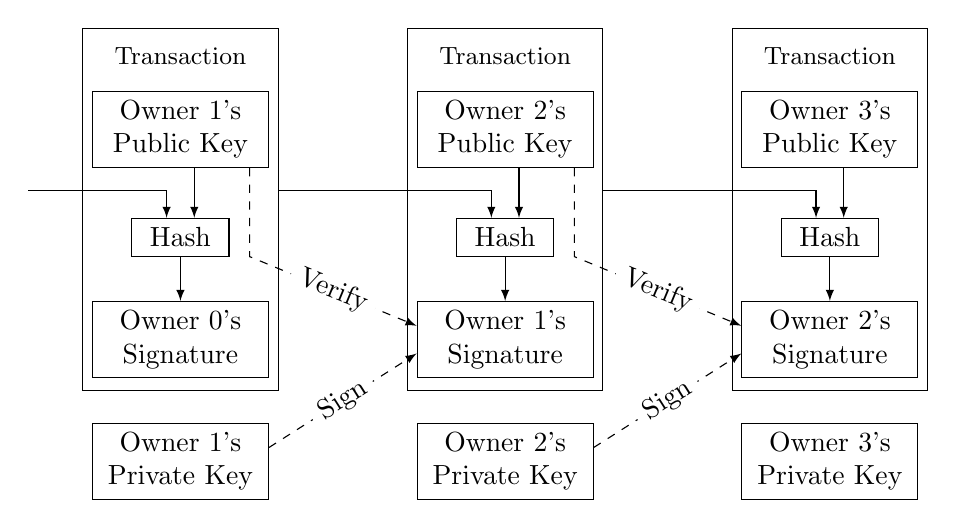
\begin{tikzpicture}[remember picture]

    % First transaction.
    \node [transaction] (t0) at (10,10) {Transaction};
    \node [key] (pubkey1) at ($(t0.south) - (0,20pt)$) {Owner 1's Public Key};
    \node [hash] (hash0) at ($(pubkey1.south) - (0,25pt)$) {Hash};
    \node [signature] (sig0) at ($(hash0.south) - (0,30pt)$) {Owner 0's Signature};
    \node (b0) [draw=black, fit={(t0) (pubkey1) ($(sig0.south) - (0,1pt)$)}] {};
    \node [key] (privkey1) at ($(sig0.south) - (0,30pt)$) {Owner 1's Private Key};

    % Second transaction.
    \node [transaction] (t1) at ($(t0.east) + (90pt,0)$) {Transaction};
    \node [key] (pubkey2) at ($(t1.south) - (0,20pt)$) {Owner 2's Public Key};
    \node [hash] (hash1) at ($(pubkey2.south) - (0,25pt)$) {Hash};
    \node [signature] (sig1) at ($(hash1.south) - (0,30pt)$) {Owner 1's Signature};
    \node (b1) [draw=black, fit={(t1) (pubkey2) ($(sig1.south) - (0,1pt)$)}] {};
    \node [key] (privkey2) at ($(sig1.south) - (0,30pt)$) {Owner 2's Private Key};

    % Third transaction.
    \node [transaction] (t2) at ($(t1.east) + (90pt,0)$) {Transaction};
    \node [key] (pubkey3) at ($(t2.south) - (0,20pt)$) {Owner 3's Public Key};
    \node [hash] (hash2) at ($(pubkey3.south) - (0,25pt)$) {Hash};
    \node [signature] (sig2) at ($(hash2.south) - (0,30pt)$) {Owner 2's Signature};
    \node (b2) [draw=black, fit={(t2) (pubkey3) ($(sig2.south) - (0,1pt)$)}] {};
    \node [key] (privkey3) at ($(sig2.south) - (0,30pt)$) {Owner 3's Private Key};

    % Coordinates for simplicity.
    \coordinate (hash0-north) at ($(hash0.north) + (-5pt,10pt)$);
    \coordinate (hash1-north) at ($(hash1.north) + (-5pt,10pt)$);
    \coordinate (hash2-north) at ($(hash2.north) + (-5pt,10pt)$);

    % Lines from transaction border to hash.
    \draw [->] ($(hash0-north) - (50pt,0)$) -- (hash0-north) -| ($(hash0.north) - (5pt,0)$);
    \draw [->] (b0.east|-hash1-north) -- (hash1-north) -| ($(hash1.north) - (5pt,0)$);
    \draw [->] (b1.east|-hash2-north) -- (hash2-north) -| ($(hash2.north) - (5pt,0)$);

    % Lines from public key to hash.
    \draw [->] ($(pubkey1.south) + (5pt,0)$) -- ($(hash0.north) + (5pt,0)$);
    \draw [->] ($(pubkey2.south) + (5pt,0)$) -- ($(hash1.north) + (5pt,0)$);
    \draw [->] ($(pubkey3.south) + (5pt,0)$) -- ($(hash2.north) + (5pt,0)$);

    % Lines from hash to signature.
    \draw [->] (hash0) -- (sig0);
    \draw [->] (hash1) -- (sig1);
    \draw [->] (hash2) -- (sig2);

    % Lines from public keys to signatures.
    \draw [dashed,->] ($(pubkey1.south) + (25pt,0)$) -- ($(hash0.south) + (25pt,0)$) -- ($(sig1.west) + (0,5pt)$)
        node [midway, sloped, fill=white] (verify1) {Verify};
    \draw [dashed,->] ($(pubkey2.south) + (25pt,0)$) -- ($(hash1.south) + (25pt,0)$) -- ($(sig2.west) + (0,5pt)$)
        node [midway, sloped, fill=white] (verify2) {Verify};

    % Lines from public keys to signatures.
    \draw [dashed,->] ($(privkey1.east) + (0,5pt)$) -- ($(sig1.west) - (0,5pt)$)
        node [midway, sloped, fill=white] (sign1) {Sign};
    \draw [dashed,->] ($(privkey2.east) + (0,5pt)$) -- ($(sig2.west) - (0,5pt)$)
        node [midway, sloped, fill=white] (sign2) {Sign};

\end{tikzpicture}
\end{document}
